\section*{Introduction (10min)}
We are studying the fifth year at computer science program at LTU and for now doing our project. As a part of our prestudy are we hosting this workshop where we will investigate possibilities through a couple of scenarios. You will do a couple of assignments in groups and then present your result and discuss these with others.

\section*{Scenario 1 (10 min + 10 min discussion)}
You have just started a course in which you will learn to program in a language that you don't find interesting. The teacher has given you a lot of recommended exercises but they don't seem very interesting. Which type of system or moments would motivate you to do the assignments. Associate freely.
\begin{itemize}
\item Which subject do you think has this problem?
\item Do the assignments need to be presented? If so, how?
\item Which material is needed?
\item If you were to make a list of highlight, what would be on it?
\end{itemize} 

\section*{Scenario 2 (10 min + 10 min discussion)}
After many years, you find yourself teaching that boring course. The boss comes in to your office late one Friday afternoon and says that the course moments are too few and that you need to update them before Monday. You sit down as the motivated teacher you are and contemplate what kind of system that would motivate students. Suddenly, you remember your old concept.

You want to make this work in the long run, which limitations must you as a teacher do?
\begin{itemize}
\item What is most time consuming?
\item Is it possible to sort your highlights by time required?
\item How many hours would be required to develop and maintain the solution over time?
\end{itemize} 

\section*{Scenario 3 15 min + 10 min discussion}
Now your system works well for that boring course and with a little tweaking, it should work with all those new courses you'll be giving. However, it is 2017 after all and the students are crying for a web-based tool. What does this tool look like? Model a web-page to fit your tool.

\begin{itemize}
\item How do you handle inputs?
\item What do your highlights look like in practice?
\item Do you see any limitations?
\end{itemize} 


\section*{Results}
\subsection*{Scenario 1}
\begin{itemize}
\item Let assignments interlink.
\item Be able to choose which assignments should be done.
    \begin{itemize}
    \item Hard to grade, every goal of the course need to be met.
    \item Assignments with similar content.
    \end{itemize}
\item Constructive alignment, how goals, assignments and examination interacts.
\item Early and quick feedback.
\item Formative assessment, continuous feedback.
\item Group assignments, hide the personal result.
\item AI Avatar that gives feedback.
\item Lot of visualization of the result.
\item Present the purpose of the assignment.
\item Different angle of the design depending on the user which is solving the assignment.
\end{itemize}

\subsection*{Scenario 2}
\begin{itemize}
\item Not everything in a course should be changed at the same time.
\begin{itemize}
\item Old assignments could be divided.
\item Shorter feedback loop.
\item Old assignments with new context.
\end{itemize}
\item Updating the course introduction is cheap and makes the goals of the course more clear when the knowledge is to be tested.
\begin{itemize}
\item Thoroughly, min/max, median or average.
\item In the end there is a written exam.
\end{itemize}
\item Retain results from previous students
\begin{itemize}
\item Keep old posts in forums.
\end{itemize}
\item Peer-to-peer feedback.
\item Test an implementation even if it's bad to receive feedback.
\item Students create assignments for each other.
\end{itemize}

\newpage
\subsection*{Scenario 3}
\begin{itemize}
\item Anonymous questions
\begin{itemize}
\item ``Did you understand what I said?''
\item Direct feedback.
\end{itemize}
\item Direct chat between students and teacher.
\item Auto generated feedback to the teacher.
\begin{itemize}
\item Aggregate data from relevant measurements.
\end{itemize}
\item A student knowledge bank.
\begin{itemize}
\item Wiki format.
\end{itemize}
\item Code correction / evaluation.
\end{itemize}

\vfill
\subsection*{Photos}
\begin{figure}[ht]
\centering
    \begin{subfigure}{.32\textwidth}
        \centering
        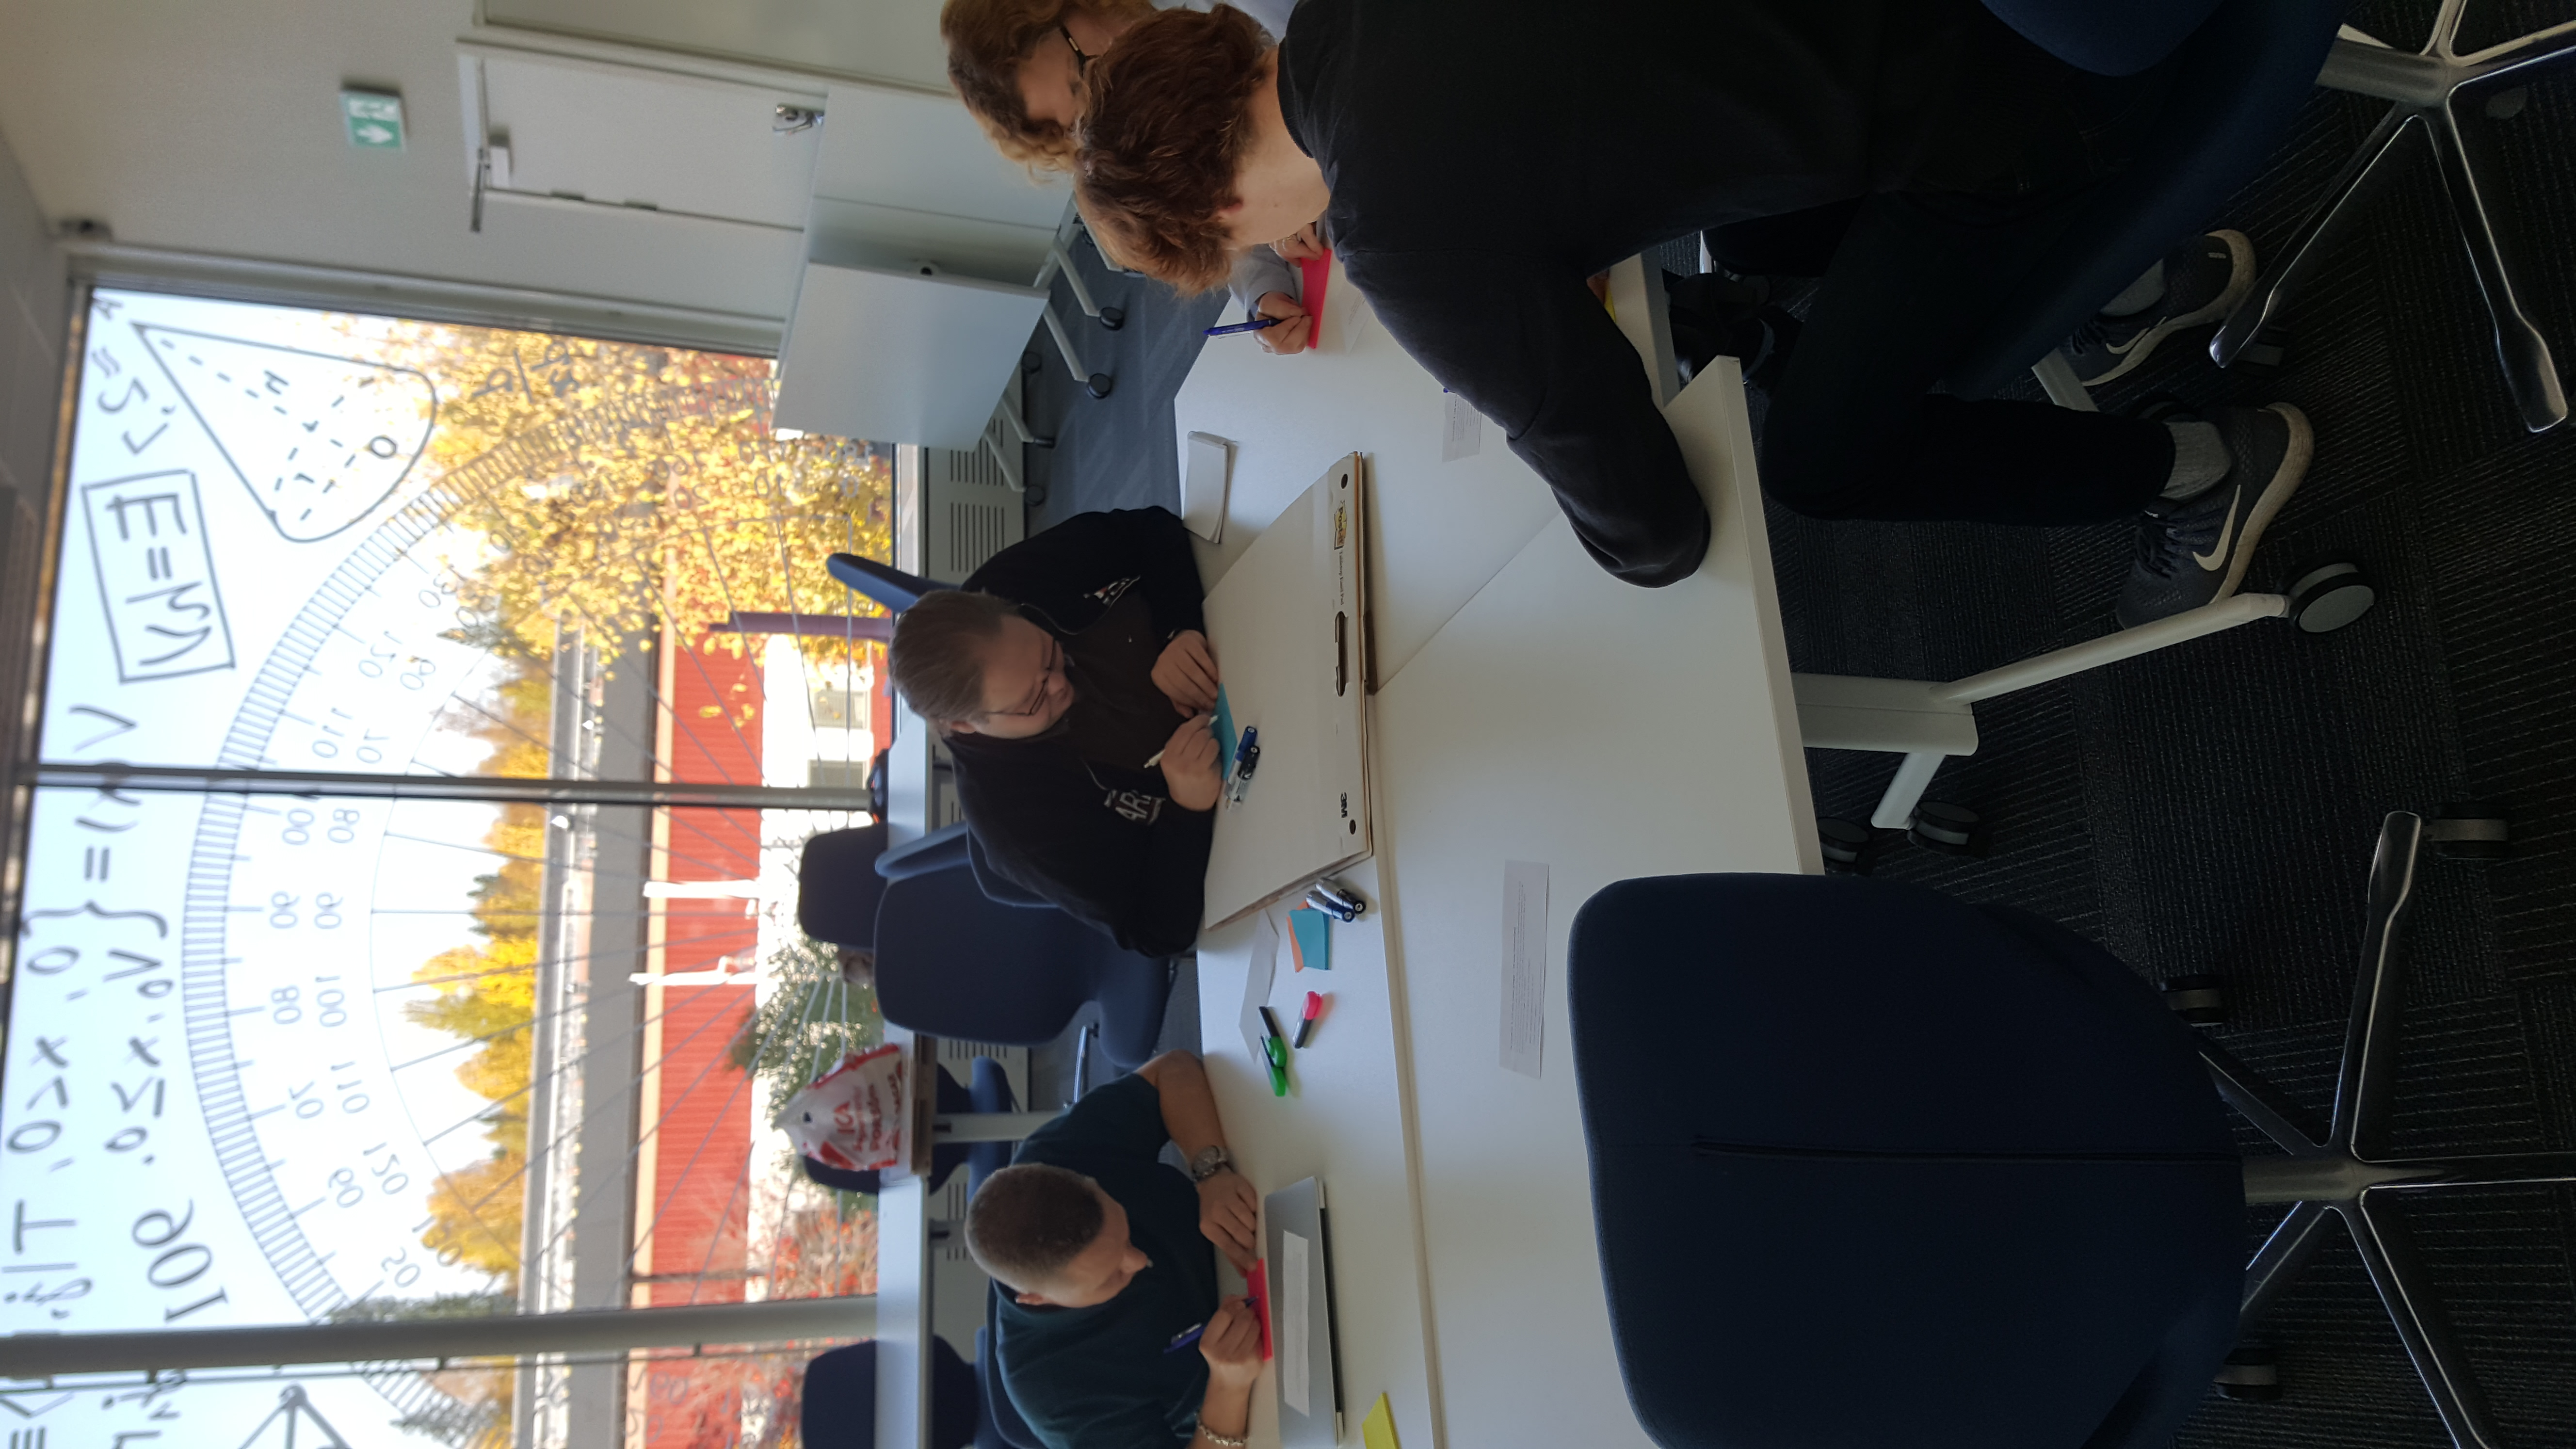
\includegraphics[width=\textwidth, angle=270, origin=c]{img/workshop1.jpg}
        \label{fig:workshop1}
    \end{subfigure}
    \begin{subfigure}{.32\textwidth}
        \centering
        \includegraphics[width=\textwidth, angle=270, origin=c]{img/workshop2.jpg}
        \label{fig:workshop2}
    \end{subfigure}
    \begin{subfigure}{.32\textwidth}
        \centering
        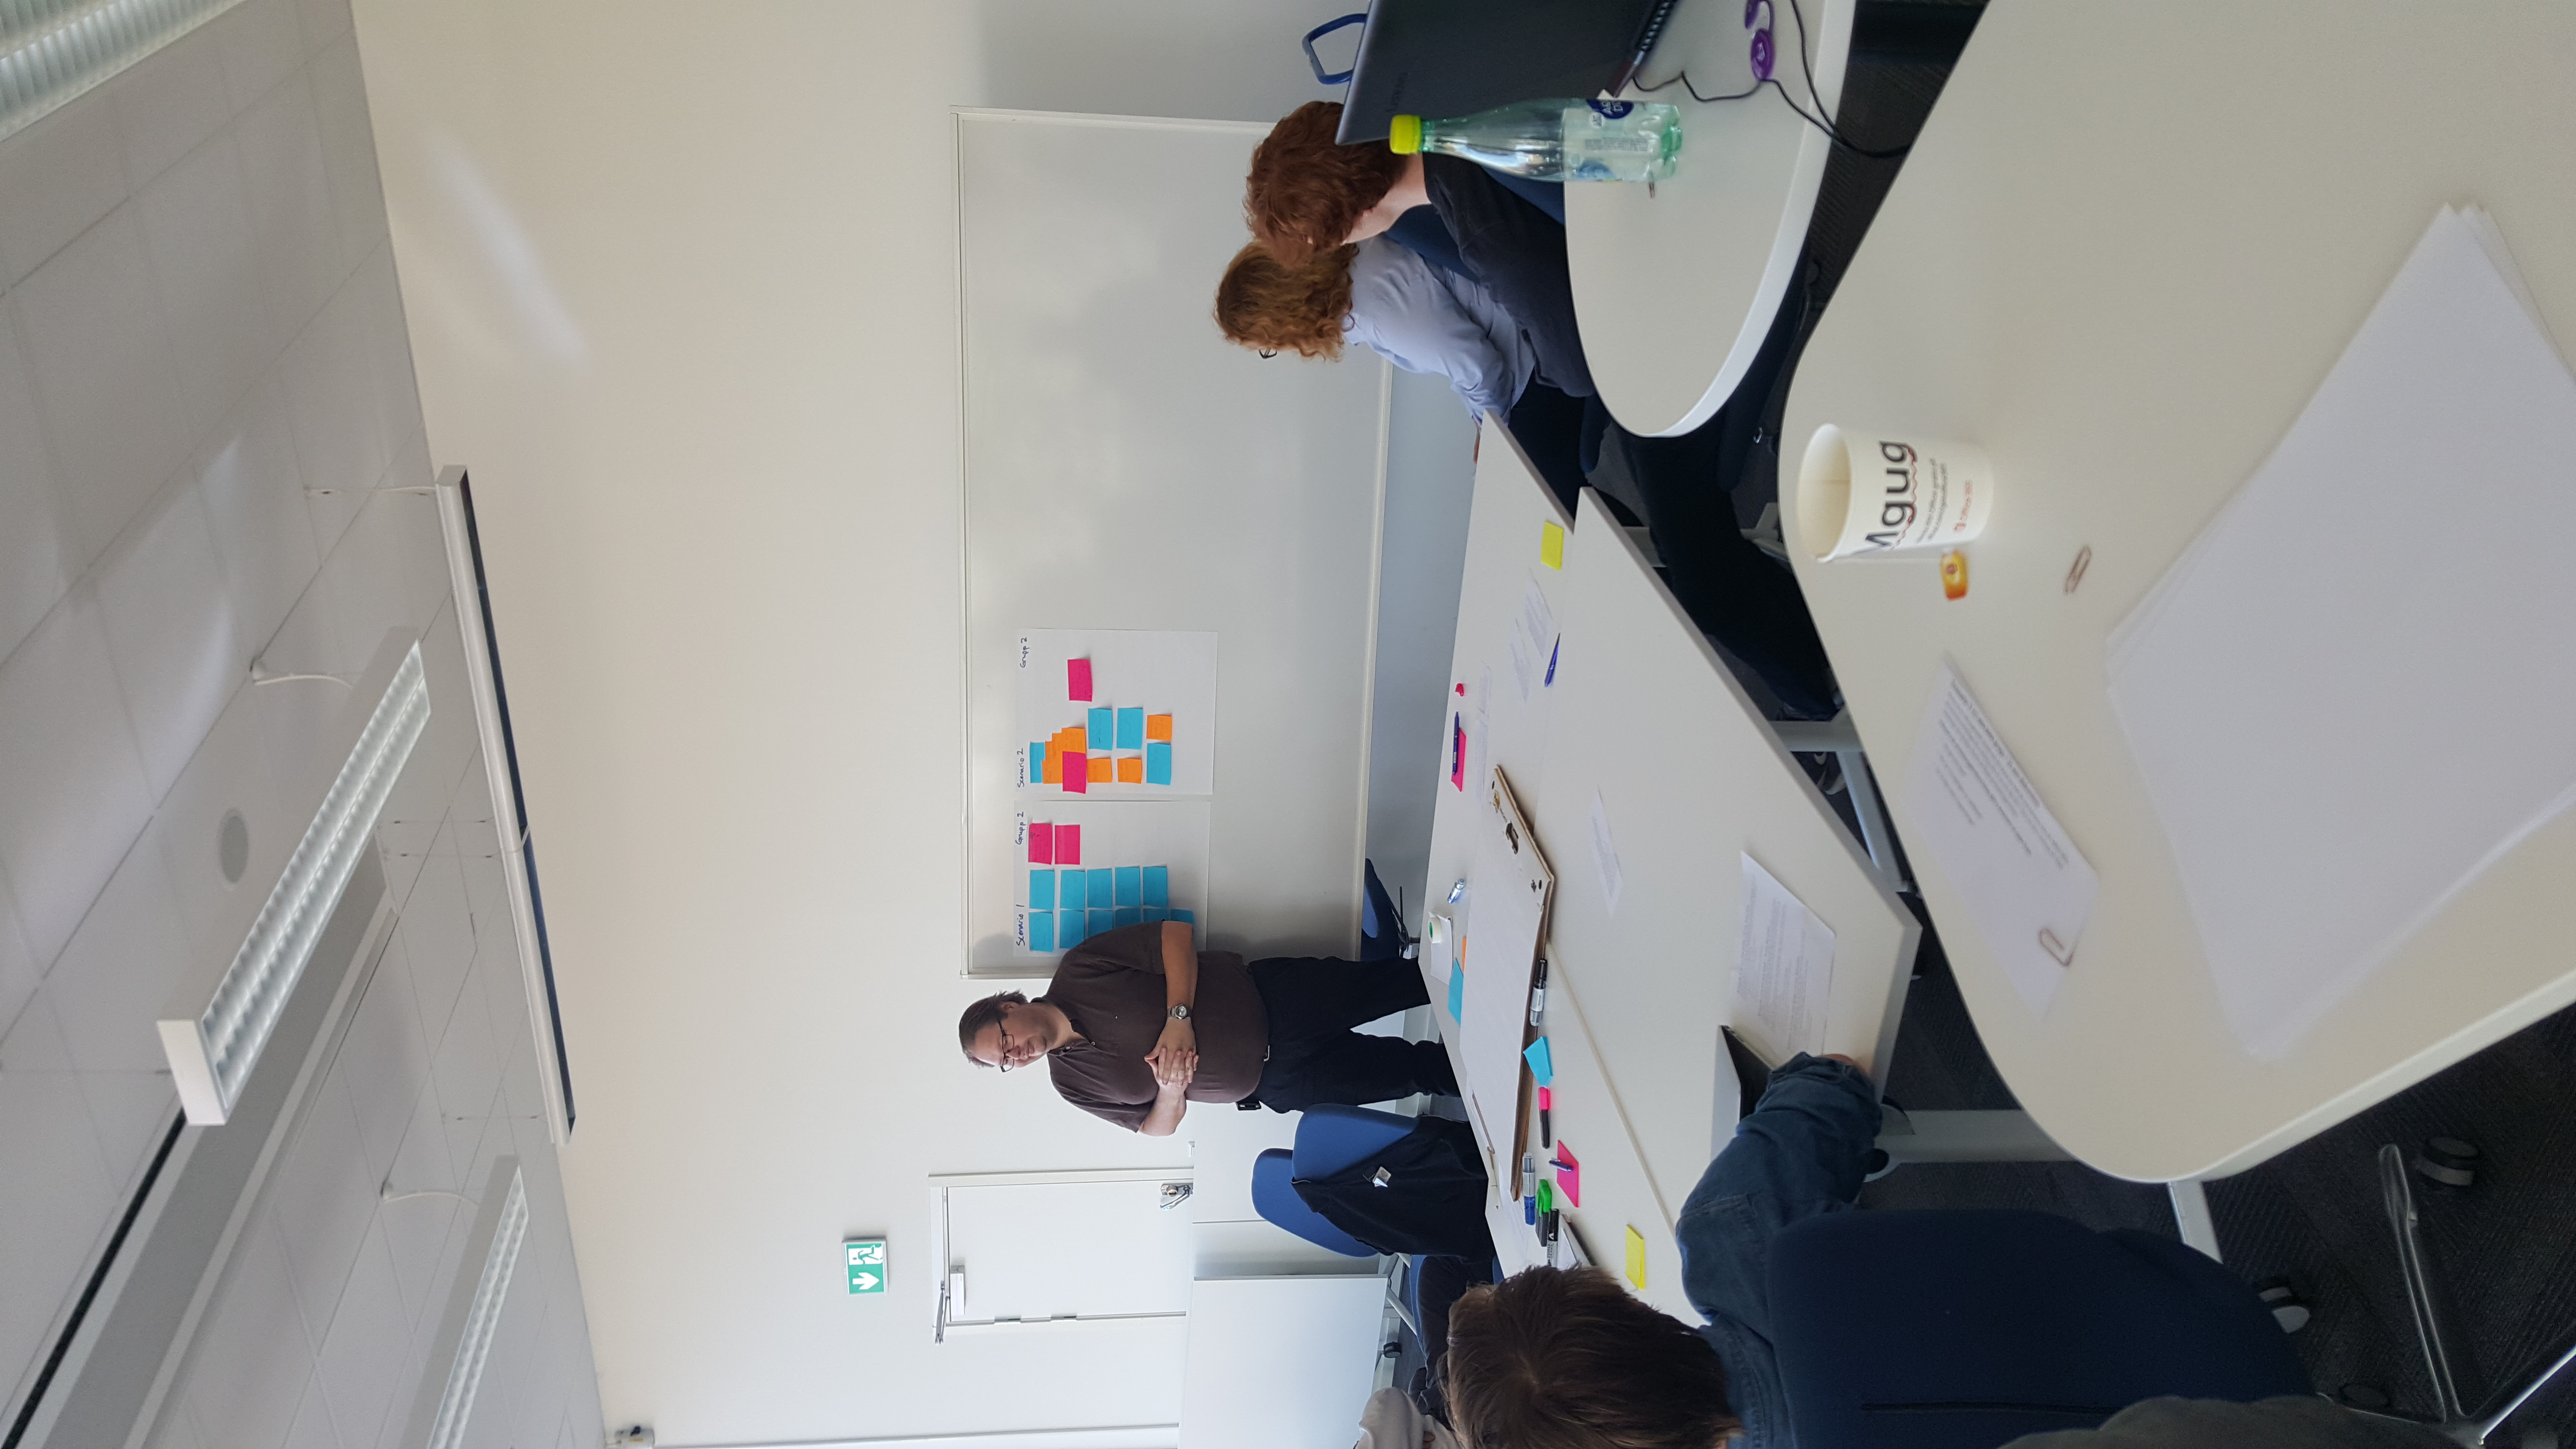
\includegraphics[width=\textwidth, angle=270, origin=c]{img/workshop3.jpg}
        \label{fig:workshop3}
    \end{subfigure}
    \caption{Workshop}
\end{figure}
\vfill

